% Physics Homework Template
% Useful for completing homework questions from the textbook.
\documentclass[11pt]{homework}
\usepackage{siunitx}
\usepackage{amsmath}
\usepackage{tikz}
\usepackage{pgfplots}
\pgfplotsset{compat=1.18}

\newcommand{\hwname}{Corbin Hibler}
\newcommand{\hwemail}{c-hibler@onu.edu}
\newcommand{\hwtype}{Ch. 19 HW}
\newcommand{\hwnum}{}
\newcommand{\hwclass}{PHYS 2311}
\newcommand{\hwlecture}{0}
\newcommand{\hwsection}{2}

\begin{document}
\maketitle

% MisConceptual Questions
\renewcommand{\questiontype}{MisConcQ}
\setcounter{questionCounter}{0}

\question
7.  D\\
10. D\\
11. D\\
12. B\\
13. B

% Problems
\renewcommand{\questiontype}{Problem}
\setcounter{questionCounter}{0}

% Problem 1
\question
\[
Q=mc \Delta T
\]
\[
6800 = (3.0)(1.000)(T_f - 10)
\]
\[
T_f = \frac{6800}{(3.0)(4186)} + 10 = \boxed{\qty{10.5}{\degree C}}
\]




% Problem 6
\setcounter{questionCounter}{5}
\question
\[
Q=mc \Delta T
\]
\[
32\,000\,000 = m(4186)(42-12)
\]
\[
\frac{32\,000\,000}{(4186)(30)} = m = \boxed{\qty{254.8}{kg / h}}
\]

% Problem 8
\setcounter{questionCounter}{7}
\question
Mass of $\qty{18}{L}$ of water is $\qty{18}{kg}$.
\[
m= \qty{18}{kg}, \quad \Delta T = \qty{80}{\degree C}
\]
\[
Q=mc \Delta T
\]
\[
Q = (18)(4186)(80) = \boxed{\qty{6.03}{MJ}}
\]


% Problem 9
\question
\[
Q=mc\Delta T
\]
\[
165\,000 = (4.1)c(37.2-18.0)
\]
\[
c = \frac{165\,000}{(4.1)(19.2)}=\boxed{\qty{2096}{J / kg \degree C}}
\]


% Problem 20
\setcounter{questionCounter}{19}
\question
\[
L_V = \qty{210}{kJ / kg},  Q = \qty{3.40e5}{J}
\]
\[
Q=mL_V
\]
\[
    \qty{3.40e5}{J} = m(\qty{210}{kJ /kg})
\]
\[
    m = \frac{\qty{3.40e5}{J}}{\qty{210000}{J /kg}}=\boxed{\qty{1.62}{kg}}
\]


% Problem 21
\question
Silver is solid at $\qty{25}{\degree C}$.
\[
m = \qty{26.50}{kg}, L_F = \qty{88}{kJ / kg} = \qty{88000}{J / kg}, \quad \Delta T = (961-25) = \qty{936}{\degree C}, \quad c = \qty{230}{J / kg \degree C}
\]
\[
Q= mc\Delta T + mL_F = (26.50)(230)(936) + (26.50)(88000) = \boxed{\qty{8.0}{MJ}}
\]


% Problem 32
\setcounter{questionCounter}{31}
\question
Isothermal means:
\[
\Delta E_{\text{int}} = 0, \quad Q = W_{\text{by}}
\]
\begin{alphaparts}
\questionpart
\[
    \boxed{\Delta E_{\text{int}} = 0}
\]
\questionpart
\[
Q = W_{\text{by}}= \boxed{\qty{4.3}{kJ}}
\]


\end{alphaparts}



% Problem 33
\question
(Generated using TikZ)
\begin{center}
    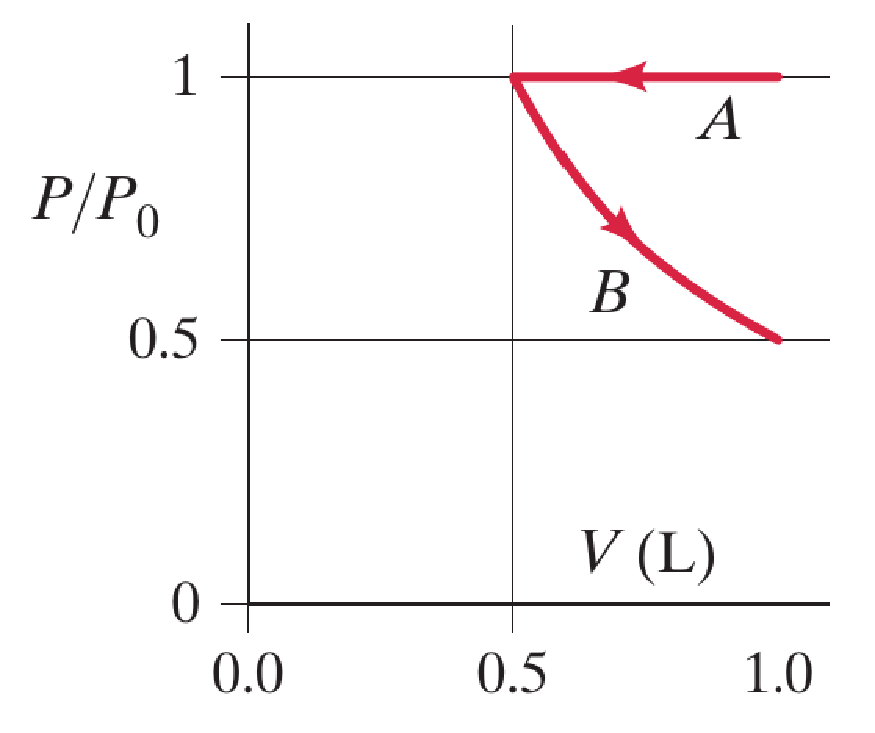
\includegraphics[width=50mm,scale=0.5]{q33.pdf}
\end{center}

% Problem 35
\setcounter{questionCounter}{34}
\question
Isobaric means:
\[
Q = \Delta E_{\text{int}} + W = \Delta E_{\text{int}} + P\Delta V
\]
\begin{alphaparts}
\questionpart
\[
W = P\Delta V = (101325)(4.1 - 2.2) = \boxed{\qty{193}{kJ}}
\]
\questionpart
\[
\Delta E_{\text{int}} = Q - P \Delta V = 680\,000 - (101325)(4.1 - 2.2) = \boxed{\qty{487}{kJ}}
\]
\questionpart
(Generated using TikZ)
\begin{center}
    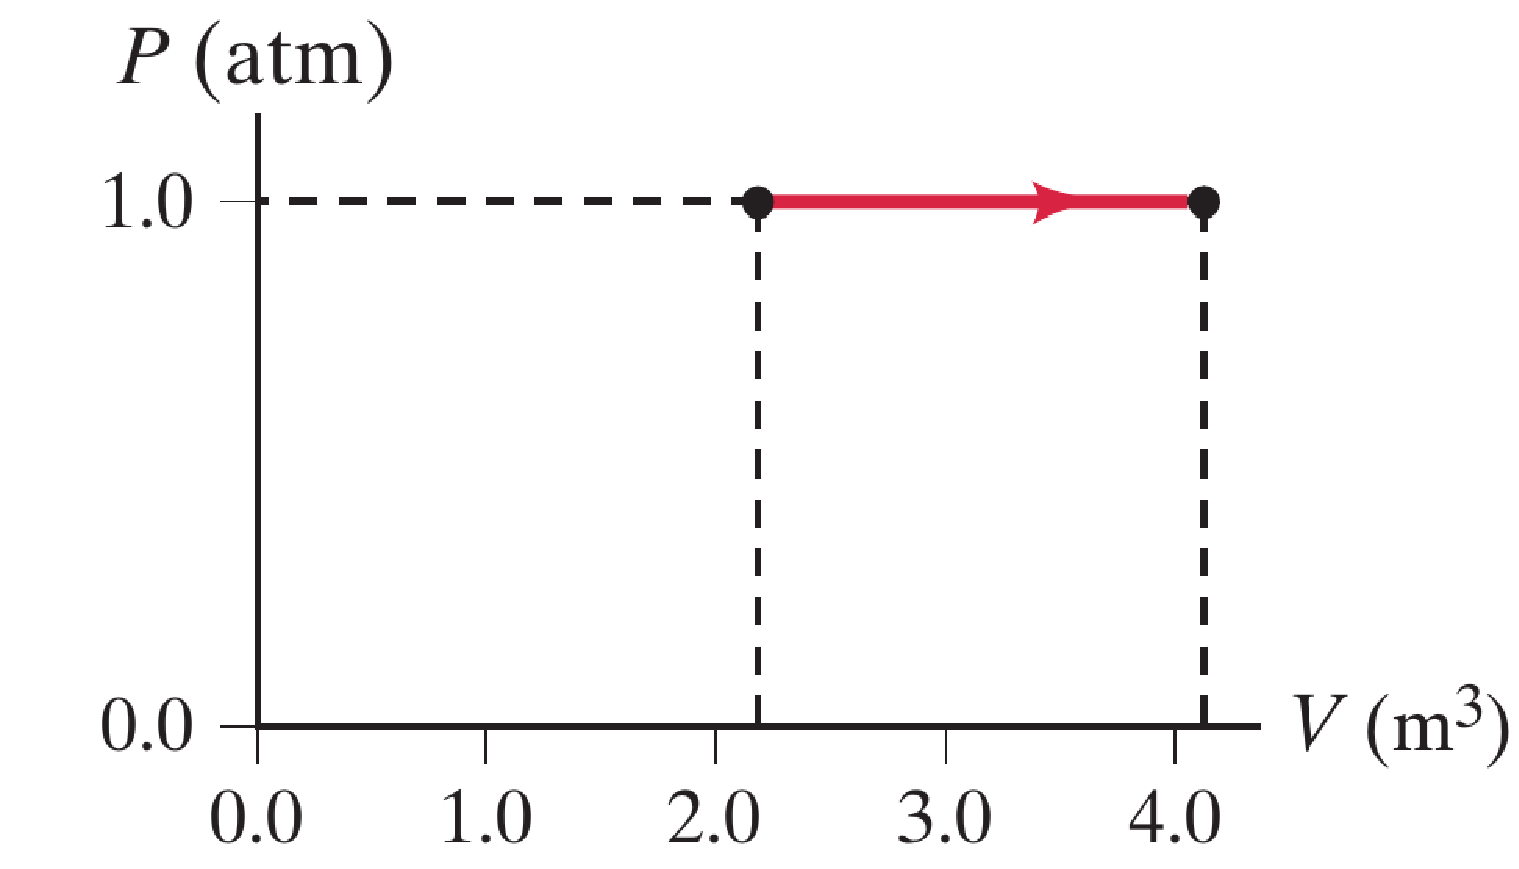
\includegraphics[width=55mm,scale=0.5]{q35.pdf}
\end{center}
\end{alphaparts}


% Problem 36
\question
Isovolumetric means:
\[
W = 0, \quad Q = \Delta E_{\text{int}}
\]
Given:
\[
Q = \qty{425}{kJ}
\]

\begin{alphaparts}
\questionpart
\[
\boxed{W=0}
\]
\questionpart
\[
\Delta E_{\text{int}} = Q = \boxed{\qty{425}{kJ}}
\]


\end{alphaparts}


% Problem 40
\setcounter{questionCounter}{39}
\question
Isothermal means:
\[
\Delta E_{\text{int}} = 0, Q = W_{\text{by}}
\]
Given:
\[
n = \qty{3.20}{mol}, \quad T = \qty{295}{K}, \quad V_1 = \qty{3.50}{m^3}, \quad V_2 = \qty{7.00}{m^3}
\]

\begin{alphaparts}
\questionpart
\[
W = nRT \ln (\frac{V_2}{V_1}) = (3.20)(8.314)(295)\ln(\frac{7.00}{3.50}) = \boxed{\qty{5440}{J}}
\]

\questionpart
\[
Q = W = \boxed{\qty{5440}{J}}
\]

\questionpart
\[
    \boxed{\Delta E_{\text{int}} = 0}
\]


\end{alphaparts}


% Problem 49
\setcounter{questionCounter}{48}
\question
Given:
\[
n=\qty{5.40}{mol}, \quad T = \qty{2450}{K}
\]
For a fully excited diatomic gas:
\[
C_V = \frac{7}{2}R
\]
\[
E_{\text{int}} = \frac{7}{2}nRT = \frac{7}{2}(5.40)(8.314)(2450) = \boxed{\qty{385}{kcal}}
\]




\end{document}
